\documentclass{sigchi}
\pagenumbering{arabic}
\usepackage{balance}  
\usepackage{graphics}
\usepackage{times}
\usepackage{mathtools}
\usepackage{amssymb}
\usepackage{url}
\usepackage{wrapfig}
\usepackage{lipsum}
\usepackage{setspace}
\usepackage{helvet}


\makeatletter
\def\url@leostyle{%
  \@ifundefined{selectfont}{\def\UrlFont{\sf}}{\def\UrlFont{\small\bf\ttfamily}}}
\makeatother
\urlstyle{leo}

% Page size.
\def\pprw{8.5in}
\def\pprh{11in}
\special{papersize=\pprw,\pprh}
\setlength{\paperwidth}{\pprw}
\setlength{\paperheight}{\pprh}
\setlength{\pdfpagewidth}{\pprw}
\setlength{\pdfpageheight}{\pprh}

% set up tight list spacing
\usepackage{enumitem} 
\setlist{nolistsep,nosep}

% for toggles
\usepackage{etoolbox}


% CHANGE FROM TOGGLE TRUE TO TOGGLE FALSE FOR NON-ANONYMOUS RENDERING
% http://tex.stackexchange.com/questions/5894/latex-conditional-expression
\newtoggle{anonymous}
\toggletrue{anonymous}
 % \togglefalse{anonymous}

% CHANGE FROM TOGGLE TRUE TO TOGGLE FALSE TO HIDE COMMENTS
\newtoggle{comments}
%\toggletrue{comments}
\togglefalse{comments}

% Comment region command (from Wesley Willett)
\usepackage[usenames]{color}
\usepackage[usenames,dvipsnames]{xcolor}
\iftoggle{comments} {
  %if we want to show comments
  \newcommand {\tim}[1]{{\color{magenta}\bf{TC: #1}\normalfont}}
  \newcommand {\cesar}[1]{{\color{NavyBlue}\bf{CT: #1}\normalfont}}
  \newcommand {\ep}[1]{{\color{violet}\bf{EP: #1}\normalfont}}
  \newcommand {\bjoern}[1]{{\color{Orange}\bf{BH: #1}\normalfont}}
  \newcommand {\jasper}[1]{{\color{Blue}\bf{JO: #1}\normalfont}}
  \newcommand {\reviewer}[1]{{\color{Red}\bf{REVIEWER: #1}\normalfont}}
  \newcommand {\neil}[1]{{\color{Green}\bf{NK: #1}\normalfont}}
}{
  %if we don't want to show comments
  \newcommand {\tim}[1]{}
  \newcommand {\reviewer}[1]{}
  \newcommand {\ep}[1]{}
  \newcommand {\bjoern}[1]{}
  \newcommand {\jasper}[1]{}
  \newcommand {\cesar}[1]{}
  \newcommand {\neil}[1]{}
}


\renewcommand{\labelitemi}{{\tiny$\bullet$}}

\usepackage[pdftex]{hyperref}
\hypersetup{
pdftitle={SIGCHI Conference Proceedings Format},
pdfauthor={LaTeX},
pdfkeywords={SIGCHI, proceedings, archival format},
bookmarksnumbered,
pdfstartview={FitH},
colorlinks,
citecolor=black,
filecolor=black,
linkcolor=black,
urlcolor=black,
breaklinks=true,
}
\toappear{CS294 Final Project Report\\Internet of Everyday Things, Spring 2015\\ Prof. David Culler}

\newcommand\tabhead[1]{\small\textbf{#1}}
\newcommand\group[1]{\textit{#1}}

\newcommand\name{SmartStorybook}
\newcommand\namesp{SmartStorybook }


\newcommand*{\layer}[1]{{\textbf{\small{\fontfamily{cmss}\selectfont{#1}}}}}
\newenvironment{myquote}{\list{}{\leftmargin=0.01\textwidth \rightmargin=0.01\textwidth}\item[]}{\endlist}
\newcommand*{\quoted}[1]{{\small{\fontfamily{cmss}\selectfont{#1}}}}
% End of preamble.

\begin{document}


\title{
\setstretch{2} \ttlfnt
\name: An Internet of Things\\
Augmented Environment Coordinator for Storytelling
\vspace{-16pt}
}

\iftoggle{anonymous}{
  %if anonymous
  \numberofauthors{1}
  \author{
  \alignauthor Anonymous for Submission\\
    \affaddr{...}\\
    \affaddr{...}\\
    \email{...}\\
  }
}{
\numberofauthors{1}
  \author{
  \alignauthor {Cesar Torres\quad}\\
    \affaddr{Electrical Engineering and Computer Sciences}\\
    \affaddr{University of California, Berkeley}\\
    \email{cearto@berkeley.edu}\\
  }
}

% % Some fancy Latex (that I copied) to make a title page banner
% \makeatletter
% \let\@oldmaketitle\@maketitle% Store \@maketitle
% \renewcommand{\@maketitle}{\@oldmaketitle% Update \@maketitle to insert...
%   \includegraphics[keepaspectratio, width=\linewidth]
%     {figures/teaser.pdf}\bigskip}% ... an image
% \makeatother


\teaser {
  \vspace{-10pt}
  \centering
    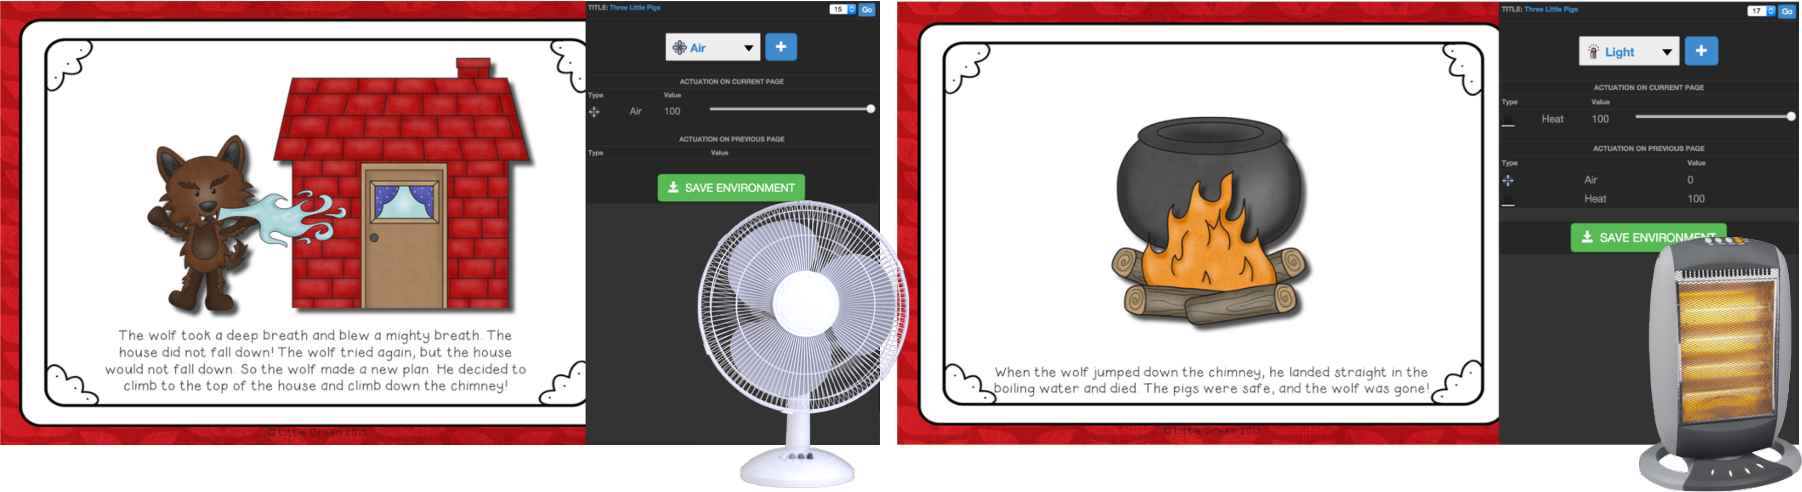
\includegraphics[width=\linewidth]{figures/teaser.pdf}
      \caption{Example story pages augmented with \name. (a) As the Big Bad Wolf huffs and puffs, a connected fan is triggered in the environment. (b) When the situation comes to a boil, a nearby heater warms the room. }
\label{fig:teaser}
\vspace{-8pt}
}
 
\maketitle

\begin{abstract}
Reading stories and experiencing storytelling is formative to a child's development and critical tool for sense-making. As the Internet of Things develops, we see new opportunities to expand the aesthetics of storytelling. We introduce SmartStorybook, an augmented environment (AE) application that controls the rich multimodal environment enabled by IoT to create interactive engagement with reading material. 
Smart Storybook contributes a content creation tool that synthesizes output with storylines. Upon reading time, the tool polls devices in a room for story enhancing capabilities (e.g. providing light, sound, smell). The desired story telling environment is resolved dynamically, providing a unique storytelling experience based on available devices and services.  
\end{abstract}


\keywords{
  internet of things, storytelling
}

\category{H.5.m.}{Information Interfaces and Presentation (e.g. HCI)}{Miscellaneous}
% \category{D.2.2}{Design Tools and Techniques}{User interfaces (H.5.2, H.1.2, I.3.6)}



%%%%%%%%%%%%%%%%%%%%%%%%%%%%%%%%%%%%%%%%%%
%%%%%%%%%%%%%%%% INTRODUCTION %%%%%%%%%%%%
%%%%%%%%%%%%%%%%%%%%%%%%%%%%%%%%%%%%%%%%%%
\newpage
\section{INTRODUCTION}
As reading technologies continue to develop, we have a new opportunity to alter and enhance the story telling experience. Story telling is fundamental to modern culture, as a means of passing knowledge and as a tool for sense-making. Interactive stories (the content) and interactive story books (the object) have been a long sought goal for human-computer interaction researchers in order to realize a long-term engagement and critical thinking. Due to the wide variety of publication mediums (print, digital, verbal) and a tension between traditional storytelling modalities, this has proved difficult. In particular, the spectacle of an augmented story book often overpowers the content and affects the learning value of the story itself. 

We present \name, a digital storybook that polls for IoT-connected devices and triggers actions based on story content. Our approach enhances the physical environment rather than imposing a virtual one. We show how this type of interface provides a seamless interaction with the storytelling experience and present novel application scenarios for improving sense-making and creating a dynamic story telling experience for repeat engagement with stories. 
   
%%%%%%%%%%%%%%%%%%%%%%%%%%%%%%%%%%%%%%%%%%
%%%%%%%%%%%%%%%% BACKGROUND %%%%%%%%%%%%%%
%%%%%%%%%%%%%%%%%%%%%%%%%%%%%%%%%%%%%%%%%%


  \begin{figure*}[th!]
      % \vspace{-8pt}
      \centering
      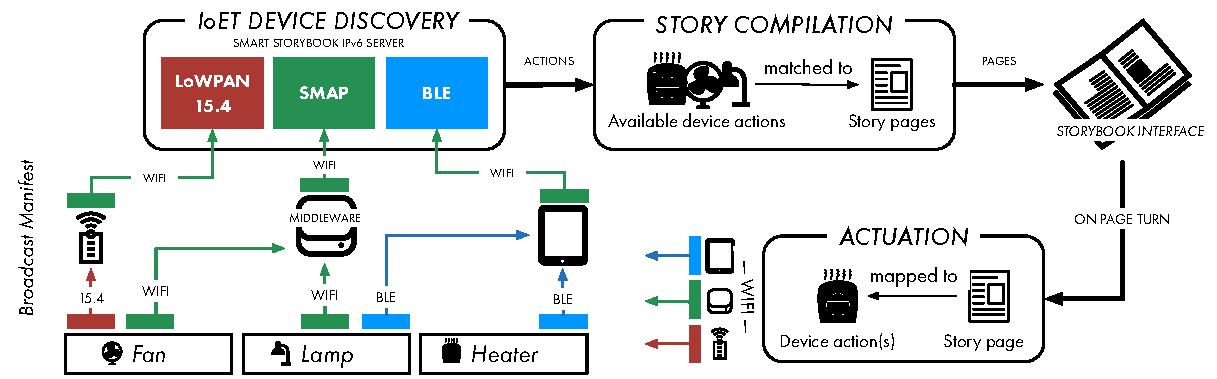
\includegraphics[keepaspectratio, width=0.98\textwidth]{figures/architecture.pdf} 
      \caption{\namesp architecture. Devices in a room broadcast available services through supported physical communication (Bluetooth, IEEE 802.15.4) in a IoET device discovery phase. A device-action list is then matched to desired actions in a story page. This story is pulled down by a storybook interface which publishes its page location. On a page turn event, the bound actions are actuated via its appropriately. }
      \vspace{-4pt}
      \label{fig:architecture} 
    \end{figure*}

\section{BACKGROUND}
The ``magic book'' has been a long sought goal for interaction researchers.
Billinghurst, et al., proposes three spheres of interaction: the tangible object, the mixed-reality universe, and the virtual universe \cite{billinghurst_magicbook-moving_2001}. Several technologies have been used to operate in each of these spaces: refined computer vision techniques have been used to prove the feasibility of an augmented reality storybook free of machine-readable markup \cite{scherrer_haunted_2008}; camera free approaches, such as Fujinami's augmented book cover and bookmark, detect page flips and offer a more mobile detection routine \cite{fujinami_page-flipping_2009}. Head-mounted displays have been shown to create immersive \textit{virtual} visual environments \cite{saso_little_2003}. Unlike mixed-reality initiatives that augment physical artifacts with virtual elements, Smart Storybook uses the StoryBubbles iPad storybook application to interface with devices and directly alter the real representation of the environment.

Other research has focused on added new interactivity to story books. 
Through simple energy harvesting, Karagozler, et al., demonstrated that powered devices can be embedded directly onto the pages of a story book \cite{karagozler_paper_2013}. A rubbing action is used to generate charge to drive LEDs and power e-paper displays and enable dynamic animations and hidden messages. 
Multimodal output have been integrated into printed artifacts \cite{iggulden_printed_1999} seen primarily in greeting cards. 

The enhanced storybook has also been examined as a method of creating a more collaborative story telling experience and enhancing the learning value of these books. Raffle, et al., demonstrated how Internet-connected storybooks could be used to create a telepresent story-telling between children and distant relatives \cite{raffle_family_2010}. The character Elmo was used to facilitate the remote interaction; however this caused attention issues since children were more prone to engage with the digital cartoon. SmartStorybook has a similar ``WOW'' factor characteristic of many new media storybooks, however we show how this is not merely a superficial element, but can be designed so children directly engage with the story content. 


%%%%%%%%%%%%%%%%%%%%%%%%%%%%%%%%%%%%%%%%%%
%%%%%%%%%%%%%%%% DESIGN  %%%%%%%%%%%%%%%%%
%%%%%%%%%%%%%%%%%%%%%%%%%%%%%%%%%%%%%%%%%%


\section{SYSTEM DESIGN}
Our architecture is composed of three major components - IoT devices (SVCD, BLE, 15.4), a middleware application used as a book repository and for content creation, and a previously developed iPad application (StoryBubbles) for viewing story content. The system architecture is depicted in Figure \ref{fig:architecture} and consists of three steps: discovery devices and services, mapping services to pages in a storybook, and actuating the necessary device through the appropriate protocol. 

\subsection{IoET Device Discovery} 
Several protocols exist for discovering devices in an environment. To allow for interoperability, we created a central repository that stores manifests for 15.4\footnote{802.15.4 6LoWPAN - Low power Wireless Personal Area Networks - a IPv6 protocol that enables small devices to have Internet-connectivity},
Bluetooth\footnote{Bluetooth Generic Attribute Profile},
and sMAP\footnote{The Simple Measurement and Actuation Profile (sMAP) is a specification for transmitting physical data to and from sensors and actuators \cite{dawson-haggerty_smap:_2010}.} 
devices. 

In this paper, we focus primarily on the actuation component of sMAP, which provides a specification for commonly used actuation patterns: binary two-state, discrete n-state, any-integer, and continuous-value actuation. A sMAP registered connected device publishes its available services to a middleware server and subscribes to a socket and listens for incoming requests. The server provides a RESTful HTTP API to get/set actuator state, while offering some rate-limiting control. 

This sMAP pattern was extended to devices published through 15.4 and Bluetooth. 
Metadata was added to published manifest for each device describing each action and its corresponding modality. 
Modality is described in terms of physical and sensory characteristics as follows: \quoted{$\langle$ light, air, sound, smell, heat, taste, motion $\rangle$}.
Each action was ascribed an amplitude (\quoted{on} $\rightarrow$ 100), and for locality a distance attribute was added to each environment. Lastly, a RESTful API set/get point was allocated to each device.

\begin{figure}[t!]
    % \vspace{-8pt}
    \centering
    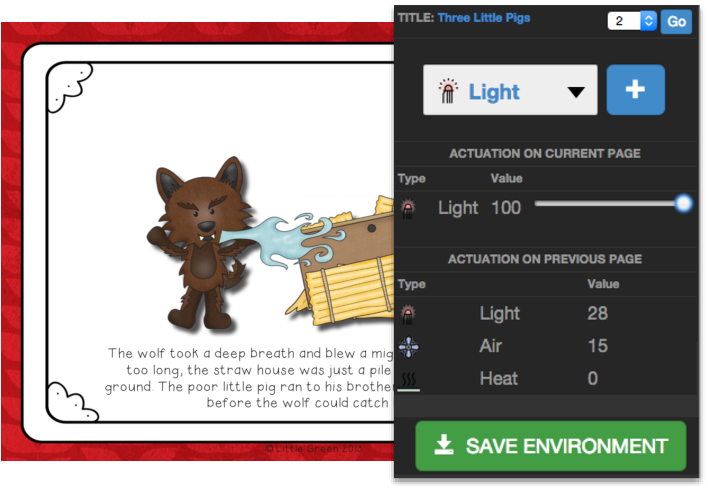
\includegraphics[keepaspectratio, width=0.5\textwidth]{figures/composer.pdf} 
    \caption{\namesp composer. Modalities are assigned to each page in the storybook to create a desired ambiance. Active page actuations are displayed to remind content authors of current conditions.}
    \vspace{-4pt}
    \label{fig:composer} 
  \end{figure}

\subsection{Story compilation}
In order to allow story developers to author interactive content into existing storybooks, we created a IoT story composer that assigns a high-level description of a desired environment to a story page (Figure \ref{fig:composer}). For each page, a story developer can specify the intensity of each modality along a continuous range from 0 to 100. For usability, active actuations (triggered from previous pages) are displayed alongside the desired environment.
\newpage
\subsubsection{Matching}
Two matching schemes were constructed to resolving devices to desired environmental or interactive conditions. 
\begin{itemize}
\item Least-squares - takes the difference in desired environment and the permutation of IoT device actions and finds the closest optimal fit. 
\item Greedy - Finds the closest modality strength value and actuate $n$ equivalent actions (e.g. $\langle$\quoted{light}, 100, $n \rangle \rightarrow$ turn on $n$ \quoted{light} actuators). 
A tuple containing UUID of the device and the name of the action was bound to the appropriate page in the story.

\end{itemize}


\subsection{Actuation}
The iPad storybook application retrieves storybook information from a server. The storybook is treated as a button stream, where each page -turn is treated as a button press event which publishes its current page number. The server subscribes to this stream, looks up linked device actions, and actuate each respective device. 
The server communicates with each protocol using a base station that ``talks'' the language of the device. For instance, BL devices are actuated using an iPad or other BL device as a relay. All device actuation logic exists in the middleware layer. 

%%%%%%%%%%%%%%%%%%%%%%%%%%%%%%%%%%%%%%%%%%
%%%%%%%%%%%%%% APPLICATIONS %%%%%%%%%%%%%%
%%%%%%%%%%%%%%%%%%%%%%%%%%%%%%%%%%%%%%%%%%


\section{APPLICATIONS}
Novel interactions exist from integrating IoT actuators to story content. In this section, we detail example scenarios for augmenting the content and experience of a story. 

\subsection{Augmented Environments}
Beyond visual animations that are present in screen-based applications, Smart Storybook interacts with a wider range of sensory experiences. By connecting to IoT devices, \name can control environmental conditions such as humidity, temperature, smell. These types of actions are generally slow actuations, taking several minutes to achieve a discriminable change. We forsee these as chapter-based interactions; whereas as more immediate changes such as air flow and ambient noise can be triggered to simulate the narrative's environment.


\subsection{Character Enhancement}
Through Smart Storybook's content creation tool, character actions can be bound to actions or to the devices themselves. In our favorite example, the wolf in the Three Little Pigs blows down the house alongside an actuated fan at high speed. These cues add theatricality to the story, a key component of engagement. Furthermore, binding an character to a device, can be used to signal character presence to young readers for a more \textit{embodied} interaction. For instance, in the story of Aladdin, the genie is either within his lamp or outside of it. A lava lamp can be bound to this condition, giving user's an indication of the genie's state and likely develop empathy through the course of the story for the genie's plight as they realize the amount of time the genie spends in his lamp. The release of the genie at the conclusion of the story could likely be signaled by a more spectacular event (such as all lights turning of flashing). 


\subsection{Dynamic Storytelling and Interactivity}
In each environment, Smart Storybook queries to find what devices are available to contribute to the storytelling experience. This means that each room has its own storytelling capabilities, and the story changes slightly with each new environment. For instance, the story Goodnight Moon, where a reader bids goodnight to the inhabitants of a room, can be made interactive such that each ``good night'' turns off an IoT device. This story would change in each room of a house, and function similarly in other locales. By retaining the novelty of stories through different augmented environments, Smart Storybook can facilitate continued engagement with readers. 

%%%%%%%%%%%%%%%%%%%%%%%%%%%%%%%%%%%%%%%%%%
%%%%%%%%%%%%%%%% EVALUATION %%%%%%%%%%%%%%
%%%%%%%%%%%%%%%%%%%%%%%%%%%%%%%%%%%%%%%%%%



\section{Evaluation}
This following example story was tested informally in a public demonstration. The audience was invited to participate in a personal interaction with a single story in the \name application or a group storytelling. 

In a mock IoET storytelling environment, our system architecture discovered up to seven connected devices. The devices included a 4-state sMAP/15.4/BL fan and a sMAP smart powerstrip with binary control to 6 devices: 3 lights, a personal heater and fan, and a scent diffuser.  

\subsection{Story: The Big Bad Wolf}
Our testing story consisted of 19-page full-page illustration of The Three Little Pigs by Little Green. Device interactions are composed in the story as follows:
\begin{itemize}
\item Firstly, a 4-state connected fan is mapped to the ``huff and puff'' of the Big Bad Wolf. As the wolf visits each respective pig's home, the fan is actuated to a higher intensity. 
\item At the introduction of each of the piglet's construction ideology, a light is turned on. For the child, this presents an opportunity to have multiple external representation (MER) important to sense-making \cite{ainsworth_deft:_2006}. 
\item Furthermore, each light is mapped to the presence of each piglet throughout the book. This acts as a cue to which characters are ``on the stage''. 
\item At the climax of the story, the wolf is thrown into a boiling pot of water. We trigger a personal heater to turn on and remain heating the environment until the conclusion of the story. 
\end{itemize}

\subsection{Results}
Due to the unexpected co-use of devices by other demonstrators, we refined the list of available devices to a single fan. Our system was able to create an augmented story with the same prior definition as above. When a heater was added to the device manifest, it was appropriately dynamically linked to trigger based on story events. 

In a personal reading setting, we quickly found that synchronousness was fundamental to the interaction. Delays in actuation would dissolve a user's ``suspension of disbelief'', or the suspension of the implausibility of the narrative. We suspect a more private setting would aid with the delay effect since evaluation of public demonstrations is more subject to its spectacle value. 

In a group setting, where one of the project authors facilitated the reading of the story, we observed that IoT actuations provided a more engaging storytelling experience especially since most of the audience where adults highly familiar with the story content. 



%%%%%%%%%%%%%%%%%%%%%%%%%%%%%%%%%%%%%%%%%%%%%%%
%%%%%%%%   LIMITATIONS & FUTURE WORK  %%%%%%%%%
%%%%%%%%%%%%%%%%%%%%%%%%%%%%%%%%%%%%%%%%%%%%%%%

\section{LIMITATIONS AND FUTURE WORK}
Adding device metadata such as proximity and context information. Many devices are proxies for actions. The granularity of their service is suspect. This can be mediated through a user selection process. 
Richer actuator control is limited by connectivity. For instance, a lightning behavior (a lamp turning on and off rapidly) is subject to the throughput of the server.
Privacy and control. During the demo, several groups were using similar devices.A similar case would likely occur in the wild; access control needs to be added to devices to prevent unwanted behavior (such as acuating a thermometer of a building). 
%%%%%%%%%%%%%%%%%%%%%%%%%%%%%%%%%%%%%%%%%%%%%%%
%%%%%%%%%%%%%%%   CONCLUSION    %%%%%%%%%%%%%%%
%%%%%%%%%%%%%%%%%%%%%%%%%%%%%%%%%%%%%%%%%%%%%%%

\section{CONCLUSION}
Smart Storybook provides an alternative viewpoint to the IoT narrative. By project touches on issues of discovery management and ensemble creation. Ultimately, ascribing relevant metadata remains the chief deterrent to widespread applicability. While the sMAP definition provides some flexibility,  there is inherently a lack of proximity information and the granularity needed for storytelling. SVCD can provide better proximity data through RSSI, or resolving devices can be made a user-process.

%%%%%%%%%%%%%%%%%%%%%%%%%%%%%%%%%%%%%%%%%%
%%%%%%%%%%%%%%%% ACK %%%%%%%%%%%%%%%%%%%%%
%%%%%%%%%%%%%%%%%%%%%%%%%%%%%%%%%%%%%%%%%%

\section{ACKNOWLEDGEMENTS}
This work was done as a CS294 class project taught by Prof. David Culler. 
Team consisted of Aparna Dhinakaran, Michael Ho, Romi Phadte. 
The StoryBubbles iPad storybook application was used with permission from Kevin Casey, and Gavin Chu. 

\balance
\bibliographystyle{acm-sigchi}
\bibliography{story}
\end{document}


